\documentclass[toc]{Template/PoS}

\usepackage{enumitem}
\setlist{nolistsep}

\title{Integrating Network-Awareness and Network-Management into PhEDEx}

\ShortTitle{Network-Management in PhEDEx}

\author{\speaker{Vlad L\v{a}p\v{a}d\v{a}tescu}\\
Caltech / USA\\
E-mail: \email{vlad@cern.ch}}

\author{Tony Wildish\\
Princeton / USA\\
E-mail: \email{awildish@princeton.edu}}

\abstract{
PhEDEx is the data placement and management tool in CMS, which controls bulk 
data-flows. While robust, its architecture is now ten years old and has yet to fully 
adapt to today's production environment, an environment in which the network is 
the fastest and most reliable component.

The ANSE (Advanced Network Services for Experiments) project, in the context of 
CMS, aims to greatly improve PhEDEx' network awareness for smart source 
selection, as well as to integrate bandwidth provisioning capabilities in the data 
transfer management. Both parts require a good knowledge of the network status, 
topology and of course, access to useful and up-to-date performance metrics.

One of the first steps towards this goal involved the identification of a mechanism 
for informing PhEDEx about independent network performance metrics. Methods 
for providing these metrics have been prototyped and verified in a LAN testbed 
using fake data transfer requests. This mechanism is already directly usable by CMS 
in their production environment.

Currently, the ANSE-PhEDEx testbed is spread over many servers at a number of 
sites. It is composed of several machines dedicated to PhEDEx site agents, one 
server holding the PhEDEx central agents, a central database and one server which 
contains the PhEDEx website and data-service. Some of the site nodes have 
additional attached storage nodes.

In this paper, we present the results of PhEDEx data transfers using the Fast Data 
Transfer (FDT) tool, on high-speed WAN circuits ranging from a few Gbps up to 40
 Gbps. We continue by discussing their implications for intelligently controlling the 
network from within PhEDEx. This involves development within PhEDEx itself, 
integration between PhEDEx and various network fabric tools, and possibly 
requirements for development of the fabric tools themselves, to support more
 sophisticated PhEDEx use-cases.

Finally, the paper will also describe the future plans for the project.}

\FullConference{International Symposium for Grids and Computing 2014

Taipei, Taiwan

25-28 March 2014}

\parindent=0pt 

\begin{document}

\section{Introduction}
PhEDEx \cite{PhEDEx} is the data-placement management tool for the CMS \cite{PhEDEx} experiment at the LHC.
%Section not numbered - will change when everything is written out
\section{Integration at the transfer level}

\subsection{Integrating FDT into PhEDEx}
The FDT\footnote{Fast Data Transfer (fdt.cern.ch)} tool integrates IDCP
\footnote{InterDomain Controller Protocol} (OSCARS)
\footnote{On-Demand Secure Circuits and Advance Reservation System} calls so
integrating it in PhEDEx naturally gives us BoD\footnote{Bandwidth on Demand}
capabilities. In addition to this, we discovered that FDT performs extremely well
as a transfer tool in itself, as we will show in this paper.

As shown in Figure \ref{fig:PhEDEx-FDT-arch}, the current architecture consists
of four main components:
\begin{description}
	\item[FDT tool] - written in Java it's based on an asynchronous, flexible 
multithreaded system, using the capabilities of the Java NIO\footnote{New I/O} 
libraries. It's capable of reading and writing at disk speed over wide area 
networks and runs on all major platforms. 
	\item[PhEDEx backend*] - written in Perl, this backend
receives transfer jobs from the FileDownload site agent which will in turn 
invoke the fdtcp wrapper. 
	\item[Fdtcp wrapper*] - written in Python this is the 
interface between PhEDEx and FDT. It prepares the file list as required by FDT, 
invokes the fdtd service and harvests reports to be propagated back to PhEDEx.
	\item[Fdtcp daemon*] - written in Python as well, it's 
a permanently running daemon, in charge with authentication and completion of requests 
from fdtcp. These requests are transmitted via PYRO\footnote{PYthon Remote Objects} 
calls and will either launch the FDT in client mode on source sites or FDT in server 
mode on destination sites.
\end{description}

The components marked with * were not developed by the same team as the one responsible 
for FDT.

\begin{figure}[h]
  \centering
  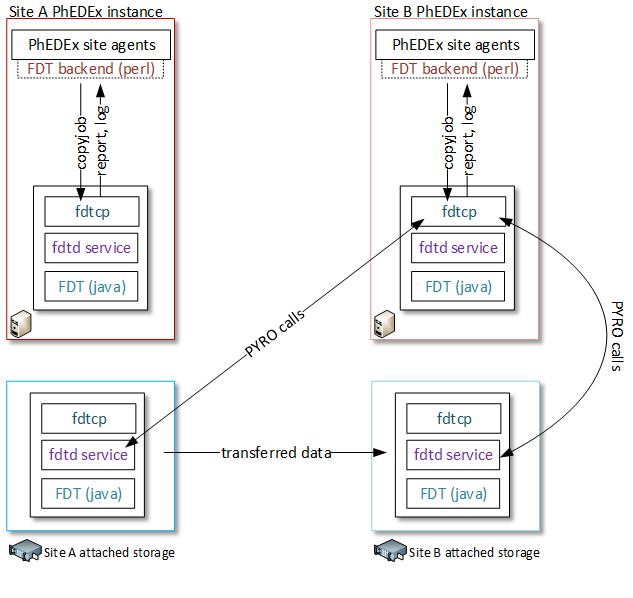
\includegraphics[width=0.95\textwidth]{Figures/PhEDEx-and-FDT-diagram.png}
  \caption{Diagram of various components needed to integrate FDT into PhEDEx}
  \label{fig:PhEDEx-FDT-arch}
\end{figure} 

Figure \ref{fig:PhEDEx-FDT-arch} also describes a normal scenario in which Site B
needs to transfer data from Site A. In this example, the PhEDEx instance and the
storage node are separate physical servers. 

Once the FileDownload agent on the PhEDEx server on Site A, marks all the files as
ready for transfer, the FDT backend on that machine will then issue an fdtcp 
command with the list of files that needs to be copied from the storage node of
Site A to the storage node of Site B.

Fdtcp will in turn, invoke the fdtd daemons on the two storage nodes. Each fdtd
daemon will first verify that the command comes from an approved server, after
which it will then launch the appropriate FDT tool. The fdtd daemon on Site B 
will start the FDT tool in server mode and the daemon on site B starts FDT in 
client mode.

Once this is done, the transfers are handled by FDT. After the transfer finishes
the reports are then propagated up the chain, eventually reaching PhEDEx.

\subsection{Setup and transfer results with FDT}

\subsubsection{Setup}

\subsubsection{Transfer results with FDT}

As seen in Figure \ref{fig:FDT-Transfers} and Figure \ref{fig:FDT-Transfers-PhEDEx}
FDT is able to achieve sustained rates of over 1500MB/sec. As PhEDEx shows,
the average sits at a marginally slower 1360MB/sec. As visible in 
Figure \ref{fig:FDT-Transfers}, the plot has periodical drops in transfer rates.
This is due to the fact that between each transfer job (which is composed of a limited
number of files) there is a delay between the ending of one job and the launch of
a new one. This is what accounts for the difference in average reported rates by PhEDEx
and the average rate for each transfer job.

These high transfer rates are not only due to the storage system alone... FDT 
automatically starts the correct number of readers and writers if the files at 
the source and destinations sites are spread on different physical disks/controllers.

\begin{figure}[h]
  \centering
  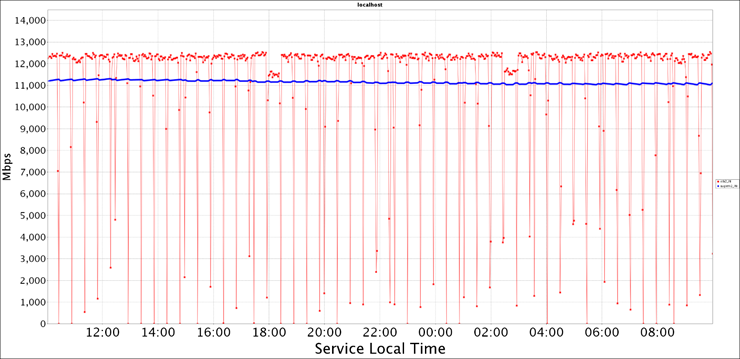
\includegraphics[width=0.95\textwidth]{Figures/FDT-transfers.png}
  \caption{PhEDEx transfers over 24hrs using FDT - MonALISA plot}
  \label{fig:FDT-Transfers}
\end{figure} 

\begin{figure}[h]
  \centering
  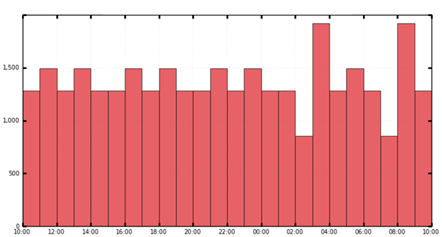
\includegraphics[width=0.95\textwidth]{Figures/FDT-transfers-PhEDEx.png}
  \caption{PhEDEx transfers over 24hrs using FDT - PhEDEx plot (in MB/sec)}
  \label{fig:FDT-Transfers-PhEDEx}
\end{figure} 


\subsubsection{Caveats}

At the moment this system does have some drawbacks:

\begin{itemize}
	\item This setup is not used by anyone in production at the moment
	\item FDT requires a POSIX compatible interface to function. At the moment
not all PhEDEx sites are capable of exposing that.
	\item In order to get the best performance out of the systems, files that
are to be transfered need to be spread among different disks on both source
and destination storage servers. This puts an additional configuration effort
on the sites and adds more complexity in the TFCs\footnote{Transfer File
Catalogs}
\end{itemize}
\section{Integration at the FileDownload Level}

\subsection{Changes to the FileDownload agent}

For this prototype we decided to integrate all of the control and circuit awareness
logic in the FileDownload agent, thus eliminating the need for an additional site 
agent or any changes to the DB schema.



\subsubsection{Making use of a circuit}

When PhEDEx transfers files, it does so in bulk. This number varies from instance
to instance, but this for PhEDEx constitutes a transfer job. Each file in a job
represents a transfer task that needs to be fulfilled. Each transfer task contains
(among others) information about the source and destination PFNs\footnote{Physical File Names}.

A PFN contains the protocol that needs to be used, the hostname or IP of the file
and the local path of that file. This means that if we want PhEDEx to use
circuits, we need a mechanism to replace the original hostname or IP in each 
source/destination PFN with the source IP and destination IP of the circuit.

Among the many events that are triggered in the FileDownload agent, a special one 
is "transfer\_task". The role of this event is to mark a task as ready for transfer. 
When all of the tasks in a particular job are ready, the backend will automatically 
launch the actual transfer of files. Since this event is triggered for each individual
transfer task, just before a transfer job is started, this is the ideal place to
substitute the original hostnames in source and destination PFNs, with the ones
that provided by the circuit API.

We modified the "transfer\_task" event and introduced additional steps before
marking task as "READY". First, we check if the link over which the file is
supposed to be transferred over has a circuit established or not. If that's the
case, we replace the hostname/IP in the source and destination PFNs with the
IPs of the circuit endpoints. Only after this is the task as marked ready for
transfer. By doing this substitution, when the transfer eventually starts
the files will be transferred over the circuit instead of the normal path. This
substitution is transparent to the rest of the PhEDEx instances and doesn't 
require any changes on other components (like the backends).

It could also happen that a circuit becomes available, while the Download agent
marks tasks ready for transfer. This means that part of the tasks in a job
will contain source/destination PFNs having the original hostname/IPs, while
others will use the circuit IPs. When the FDT backend is used, it will automatically
launch two different jobs: one for the files transferred over the normal path
and the other for files transferred over the circuit. We still need to test
how the other backends react. In any case, even if a transfer job would fail 
because of this, PhEDEx will just try and the transfer would succeed the second
time.

\subsubsection{Circuit awareness and lifecycle management}

Since the standard FileDownload agent doesn't have knowledge about more than one
transfer paths over a given link we needed to add this circuit awareness and a
way to manage the lifecycle of a circuit on a given link.

Because of this we added several POE controlled events. Here are the main ones:

\begin{itemize}
  \item check\_workload
  \item request\_circuit
  \item handle\_request
  \item teardown\_circuit
  \item check\_circuit\_setup
\end{itemize}

\paragraph{check\_workload}

This is a recurrent event at 60 second intervals. It is used to estimate the 
amount of work that remains to be done based on the current size of the download
 queue. In order to do this, it needs to know the average rate that the current 
link is capable of and the total number of pending bytes. The latter is calculated
based on the PENDING tasks that it currently holds. The former can be retrieved
in two ways: 

\begin{itemize}
  \item if the agent has recently transfered tasks it will retain information about
previously DONE tasks, which will then be used for the average rate calculation
  \item if nothing has been transferred, it will try to get this information based
on the link average rate calculated by PhEDEx itself.
\end{itemize}

If an average rate source-destination pair has been calculated, it will estimate
the amount of work needed to be done.

If for a given link the following are true, a circuit request will be made:
\begin{itemize}
  \item the amount of work pending is above a given amount (currently 5h worth of transfers) 
  \item a circuit has not been established
  \item a circuit request is not pending
  \item a circuit request hasn't previously failed
  \item transfers haven't previously failed while a circuit was active
\end{itemize}

\paragraph{request\_circuit}

As the name suggests this event is used to request a circuit.

It will:
\begin{itemize}
  \item create a state file for this request in "state/circuits/request". 
This file contains PhEDEx nodes involved in request, time of request and the 
lifetime of the circuit.
  \item starts a timer to the event "handle\_request\_timeout". If we don't
get a request within 10 minutes it's very likely that we won't get it at 
all.
  \item in the case of this prototype "handle\_request" is called directly,
however in the production version, this event will actually be a callback
from the API call where a circuit is being requested
\end{itemize}

\paragraph{handle\_request}

This event is a callback from the API call to request a circuit.

It will:
\begin{itemize}
  \item trigger the event "remove\_circuit\_request"
  \item if the circuit creation failed, flag it and return from event
  \item modifies and saves the state file corresponding to this request by 
adding relevant information concerning the circuit that has just been established:
time the circuit was established, time the circuit expires, endpoint IPs of 
the established circuit.
  \item starts a timer to the event "teardown\_circuit" if an expiration
time has been specified for the circuit
\end{itemize}

\paragraph{check\_circuit\_setup}

This is another recurrent event at 60 second intervals and is used to provide
sanitation in case of errors. An important scenario is what happens after an
agent crashes and is restarted. If such a thing occurs, there are two possible
cases:

\begin{enumerate}
  \item Download agent has crashed
  \begin{enumerate}
    \item Internal data is lost, but state file(s) exist in circuits/requested:\\
			If there's a state file in /circuits/requested but no matching internal data, 
			try to cancel the request and remove the file from the folder
    \item Internal data is lost, but state file(s) exist in circuits/established:\\
			If there's a file in circuits/established, but no matching internal data:
			check the expiration time in the state file:
			\begin{itemize}
			  \item if the expiration time is not defined, or is defined but didn't expire yet,
					  the circuit can be reused. Internal data is populated based on state
					 file and if the expiration time is defined, the teardown\_circuit timer is
					 triggered.
			  \item if the expiration time is defined at it expired, remove the state file and
					 try to tear down the circuit 
			\end{itemize}
  \end{enumerate}
  \item Reconsider failed circuits with failed requests or transfers:\\
		  Creating a circuit on a particular link may have been blacklisted due to requests
		  for circuits failing or due to files transfers failing on that circuit. After a given
		  time these circuits are removed from the blacklist and the system is free to try
		  and use them again.
\end{enumerate}

\begin{description}
	\item[handle\_request\_timeout] \hfill \\
		Event triggered after a timeout, it's used to cancel request and clean internal state
	\item[remove\_circuit\_request] \hfill \\
		Cleans up internal data and state file concerning this request
	\item[teardown\_circuit] \hfill \\
		Cleans up internal data and state file concerning the circuit and calls API for 
		tearing down the circuit.
\end{description}

\subsection{Setup and test}
The prototype was tested on ANSE's testbed (Figure \ref{fig:testbed}) using 
two sites: T2\_ANSE\_Amsterdam and T2\_ANSE\_Geneva. These sites consist of two
 servers each: a PhEDEx server and a dedicated storage server for that particular 
 PhEDEx instance. Each of the two storage servers consist of dual 8 core CPUs 
 (with HT), 64GB of RAM and 2 LSI controllers which manage 8 SSDs each. We created 
 two RAID-0 partitions of 4 SSDs each on every LSI controller. Since the tests are write 
 intensive and were scheduled to run for around 24 hours, we decided to only use 
 1 controller, in order to minimize the negative effects on the lifetime of the disks.

The two sites were connected via a high speed 40Gbps link. On this link we could create
static virtual circuits and for the purposes of our test we decided to create two new
circuits of 10 Gbps each.

One of these circuits was used to model a shared link in which PhEDEx had to compete 
with other traffic. This background traffic was generated by Iperf and consisted of a 
continuous stream of UDP packets at 5Gbps . The other circuit served as the dedicated
link.

Monitoring was done with MonALISA\footnote{MONitoring Agents using Large
 Integrated Services Architecture (monalisa.cern.ch)} and the PhEDEx tool itself.

The main purpose of this test wasn't to show that we can saturate a 10Gbps link with
PhEDEX (although we came close with just 1 controller), but that a PhEDEx instance 
is able to switch to using a new path in a transparent manner for the other instances
and with no down time. 

The first part of the test consisted of a 10 hour run with PhEDEx transfers on the 
shared link. After this time, PhEDEx switched to using the dedicated circuit and
continued transfers for another 10 hours.

We set up PhEDEx to run a single 450 GB transfer job at a time, each one 
comprising of 30 files of 15 GB each. 

\begin{figure}[h]
  \centering
  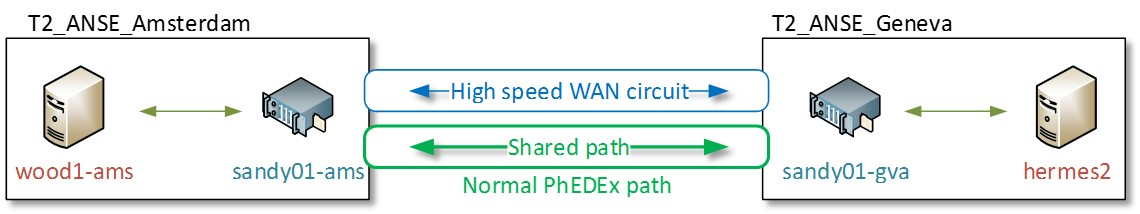
\includegraphics[width=0.95\textwidth]{Figures/FileDownload_ANSE_Testbed}
  \caption{Diagram of the testbed used by the prototype}
  \label{fig:testbed}
\end{figure} 
\

\subsection{Results}

The results of the first half of the test are shown in  (Figure \ref{fig:shared_transfers}).
A quick glance at this plot, shows that the 10 Gbps link was saturated by the two
competing transfers. Between 23:00 and 0:00 (beginning of the plot) and 
10:00 and 11:00 (end of the plot), only UDP traffic was sent across the network, 
running at a steady 5 Gbps. This effectively leaves only 5 Gbps of PhEDEx traffic.
PhEDEx transfers start around 0:00 and quickly saturate the 10 Gbps. 
The seesaw look of this plot is due to the fact that PhEDEx has a delay
between finishing one job and starting the next. This is due to various factors:
 pre/post validation, preparation of copyjobs or even time spent by the backend itself 
 before actually launching a transfer. Because of these delays, the average 
 rates reported by PhEDEx will always be lower than the average rates of each
 individual transfer job. Nevertheless we get average transfer rates of 9.5 Gbps for the
 whole link and consequently 4.5 Gbps for PhEDEx transfers (10\% penalty from
 gap between jobs).

\begin{figure}[h]
  \centering
  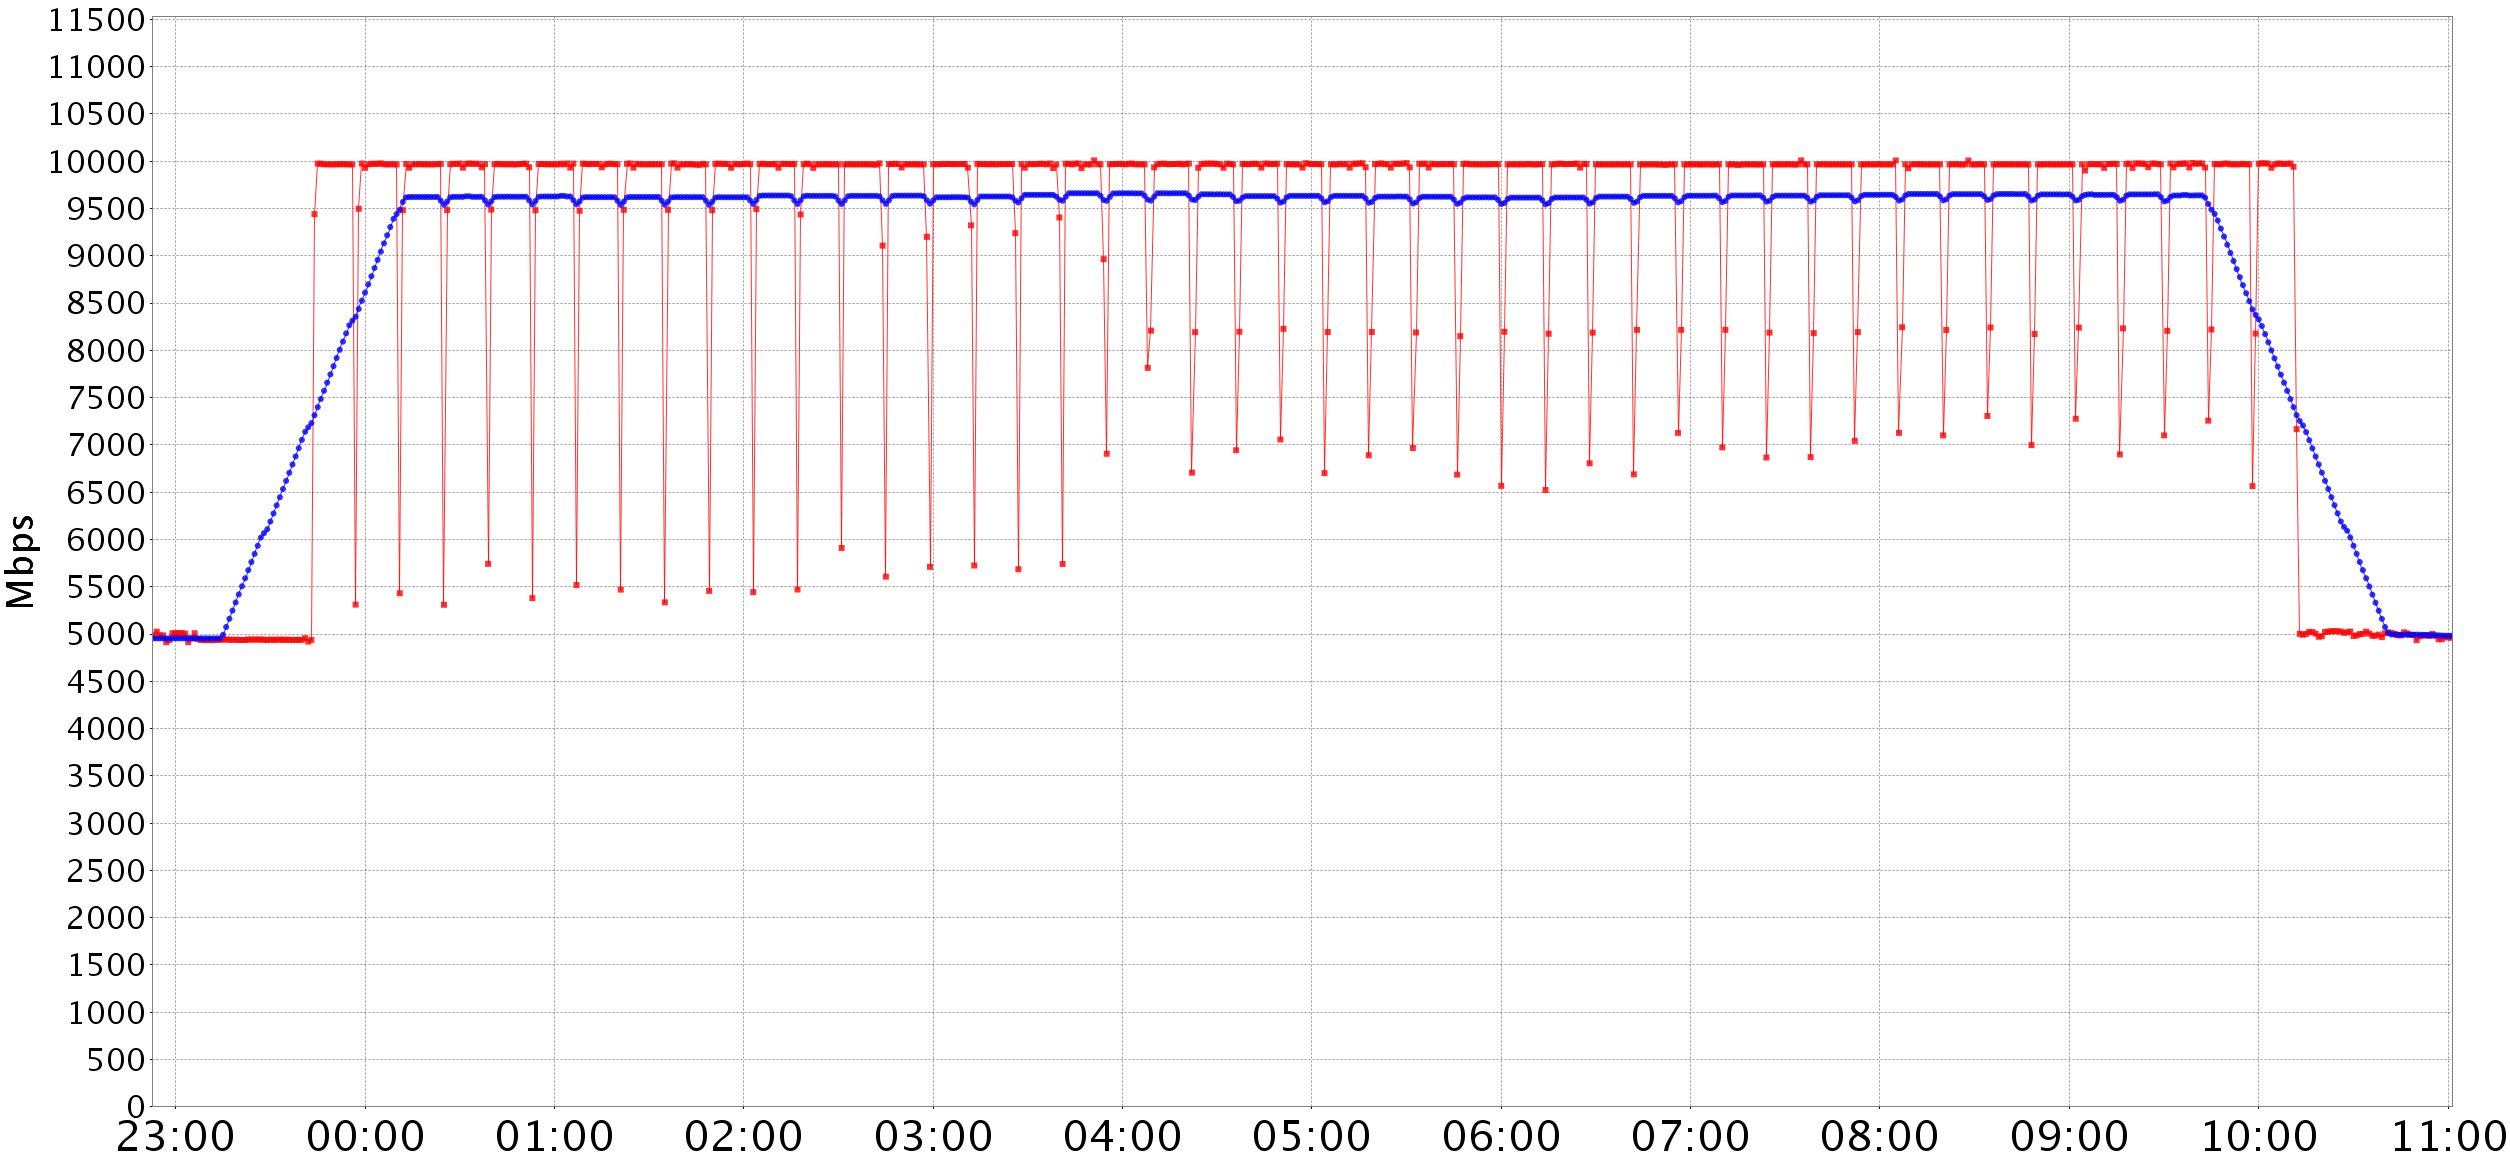
\includegraphics[width=0.95\textwidth]{Figures/FileDownload_Shared_path.png}
  \caption{PhEDEx transfers on the shared path - competing with 5Gbps UDP traffic}
  \label{fig:shared_transfers}
\end{figure} 

Around 10:00 PhEDEx switches to using the dedicated link. The results of the 
second half of the test are shown in Figure \ref{fig:solo_transfers}.

Although most of the time we are able to saturate the 10Gbps link with PhEDEx 
traffic alone we sometimes see dips in transfer rates. These dips can be attributed 
to the storage not being able to sustain such high write rates.

This time, the average link rates drop from 9.5 Gbps to 8.5 Gbps, however 
actual PhEDEx transfers go up from 4.5 Gbps to 8.5 Gbps! The reason for this 
drop in average link rate is two fold: 

\begin{itemize}
  \item Transferring a job at higher speeds means that it will take less time for
  it to complete, hence more jobs will be completed in one hour. However, as
  we previously explained, there is a delay before starting each new job, which
  means that more delays will be introduced into the system.
  \item The storage system (using 1 LSI controller) sometimes cannot sustain
  write rates of 10 Gbps to disk.
\end{itemize}


\begin{figure}[h]
  \centering
  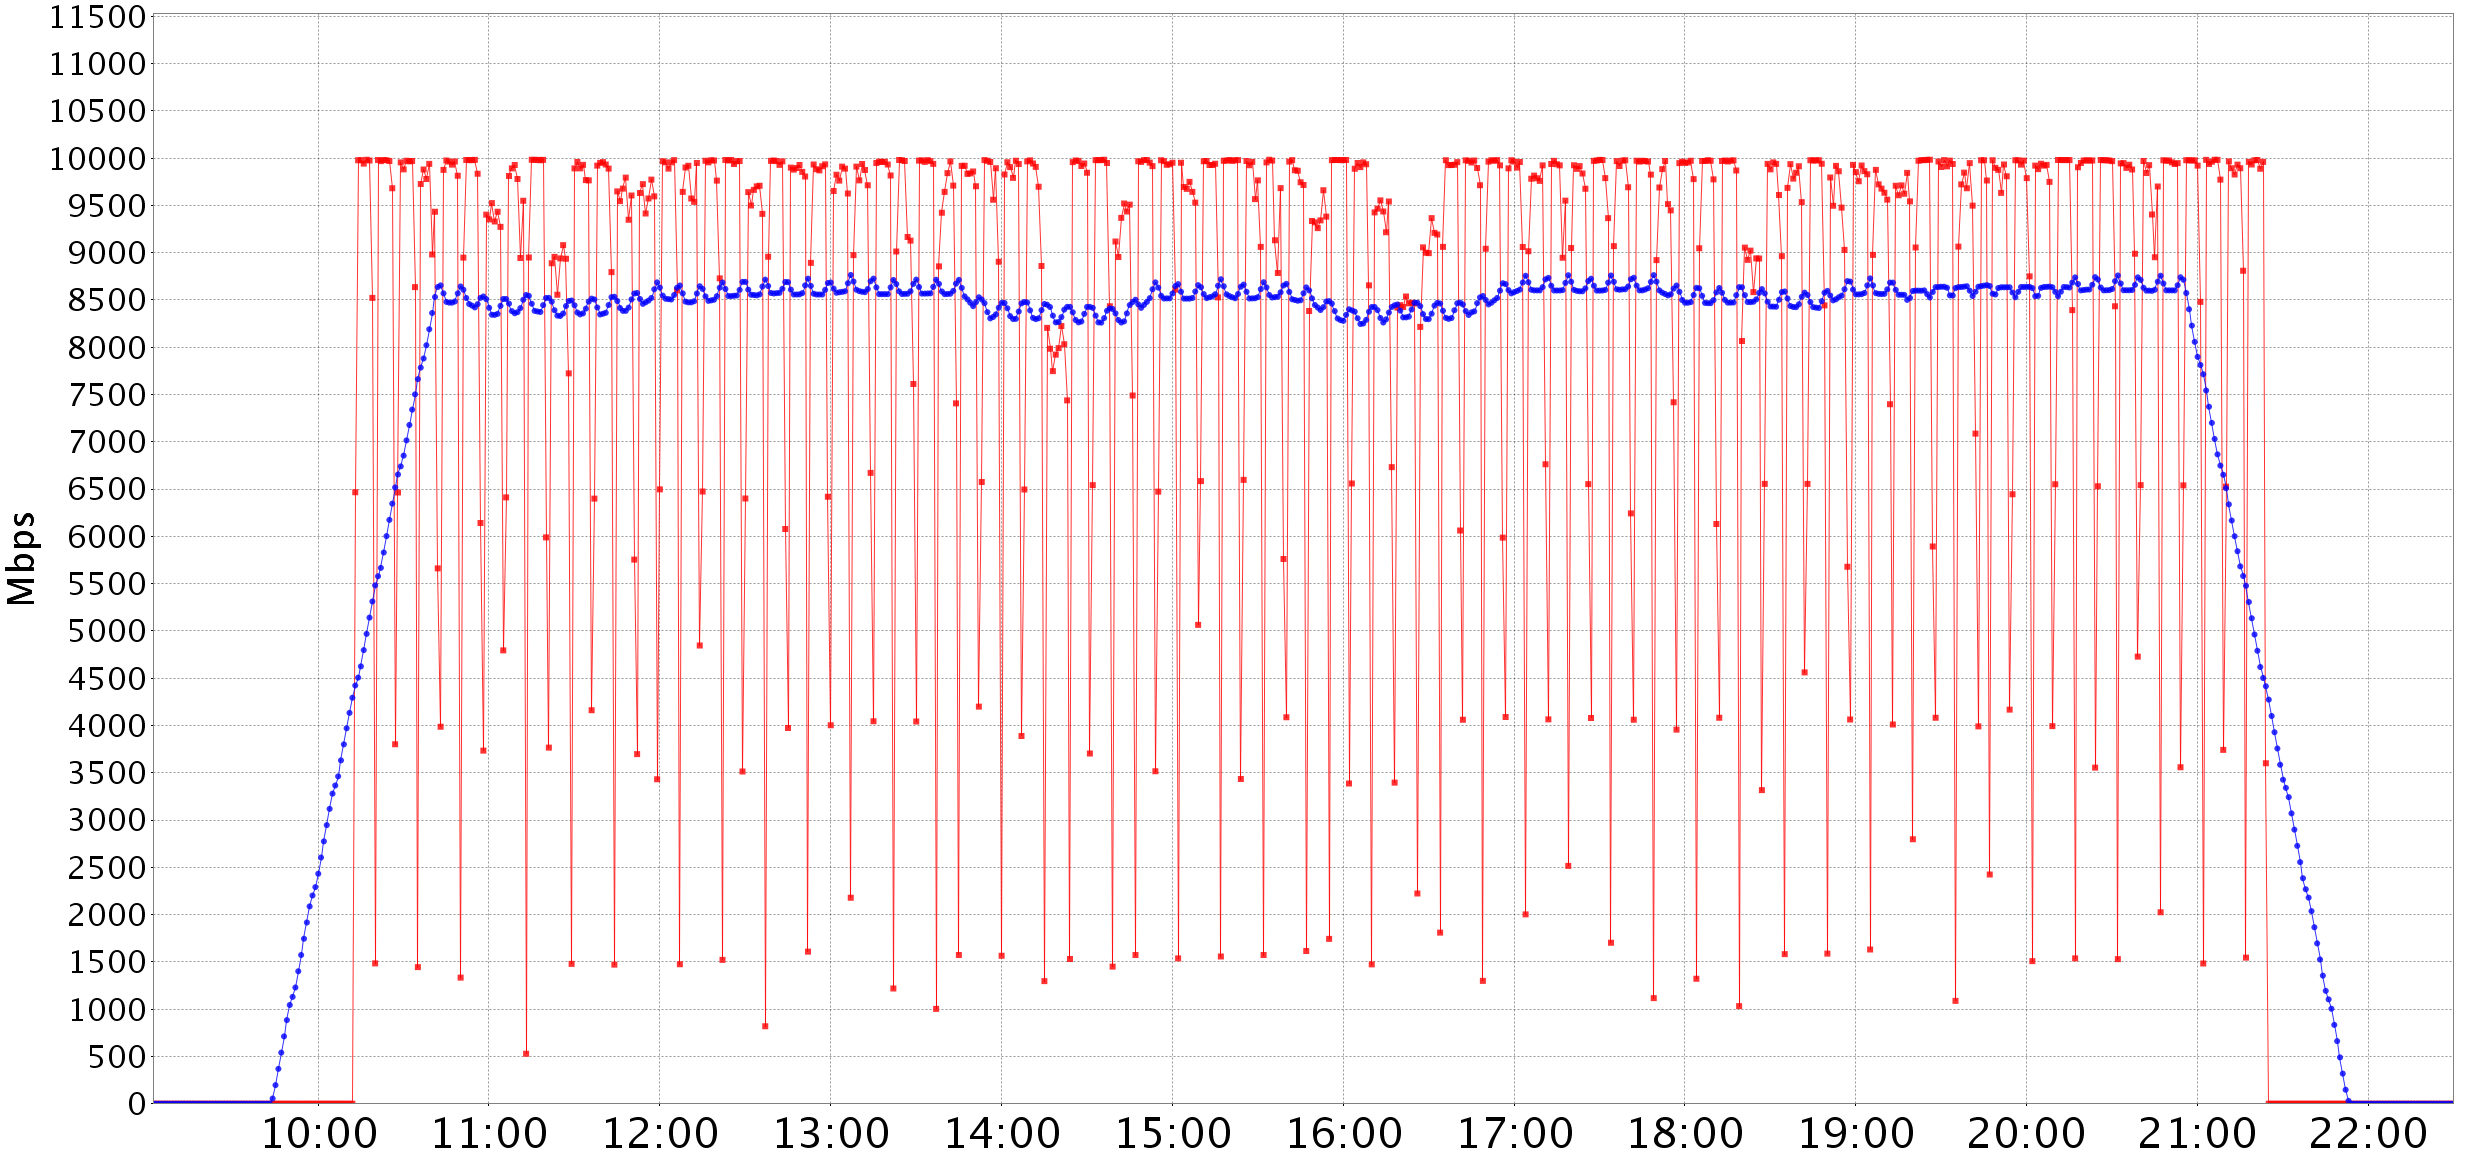
\includegraphics[width=0.95\textwidth]{Figures/FileDownload_Solo_path.png}
  \caption{PhEDEx transfers on the dedicated path}
    \label{fig:solo_transfers}
\end{figure} 

Figure \ref{fig:combined_transfers} and Figure \ref{fig:combined_phedex_transfers} show
the  network activity for PhEDEx traffic alone on both links. 
In this plot we can observe that PhEDEx switches to using the
new link without any interruption in service, doing it seamlessly and in a 
transparent way for the other instances (switch occurs around 10:00).

This plot also shows that there is a huge benefit to using the dedicated link.

\begin{figure}[h]
  \centering
  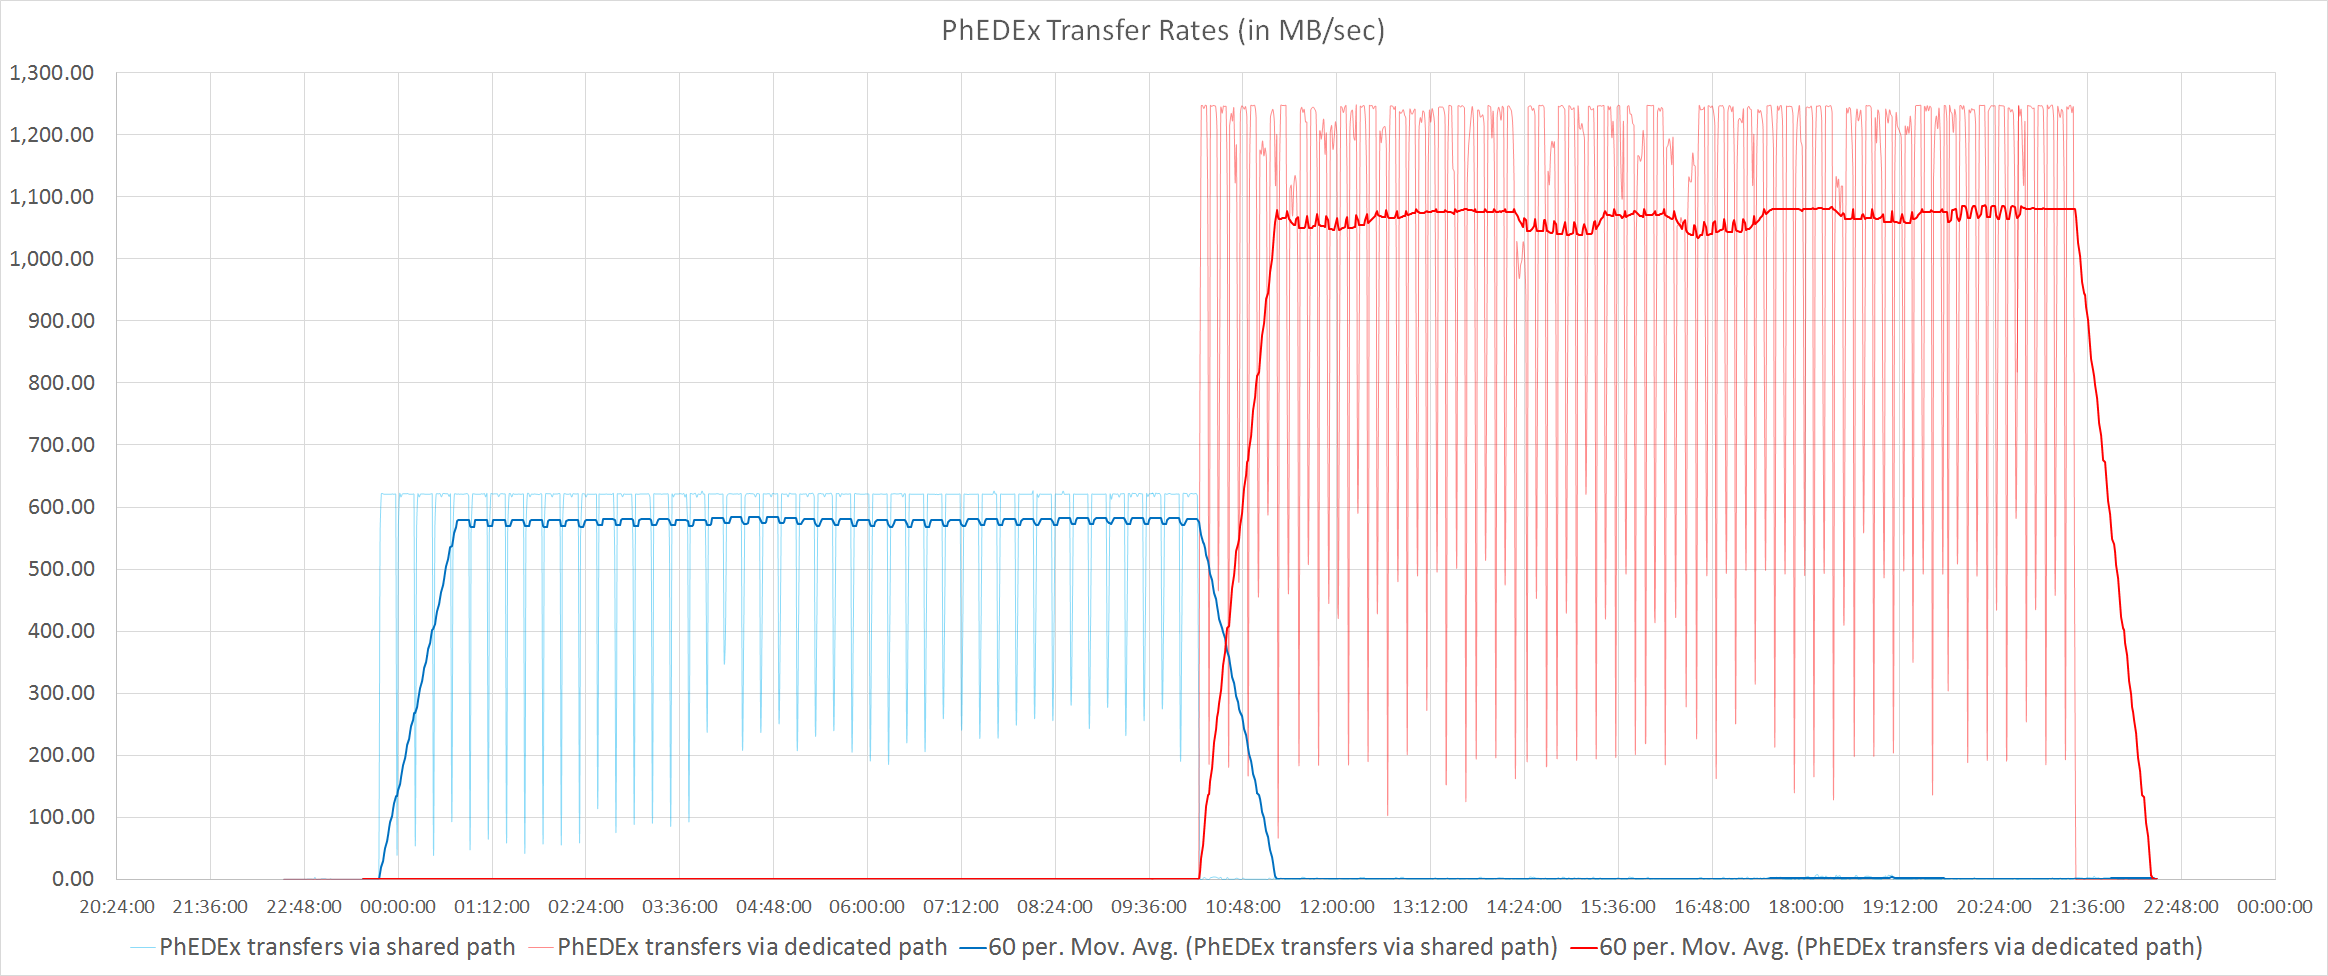
\includegraphics[width=0.95\textwidth]{Figures/FileDownload_All_paths.png}
  \caption{View of PhEDEx only transfers on both the shared and dedicated path}
  \label{fig:combined_transfers}
\end{figure} 

\begin{figure}[h]
  \centering
  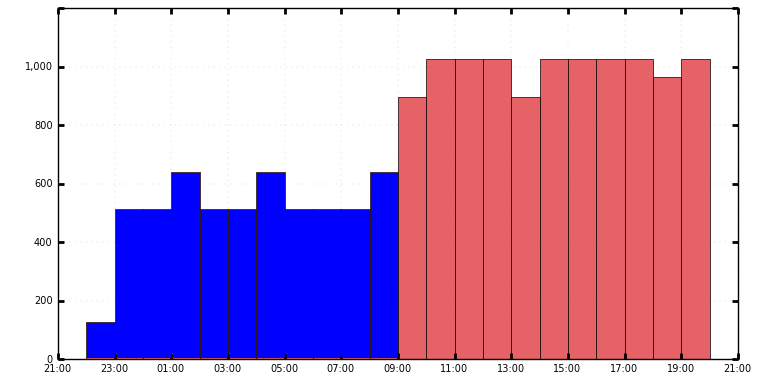
\includegraphics[width=0.95\textwidth]{Figures/FileDownload_PhEDEx_all_paths.png}
  \caption{View of PhEDEx only transfers on both the shared and dedicated path}
  \label{fig:combined_phedex_transfers}
\end{figure} 
%% Vlad, this is for you
\section{Summary}
main points to bring out:

CMS intends to integrate network-awareness into PhEDEx. We have a prototype that transparently integrates the use of virtual-circuits in the FIleDownload agent. The next step is to interface to the circuit API, so the agent can directly control the circuits. After that, proceed to integration at the FileRouter level.

%% Tony will set this up

%% \section*{References}

\begin{thebibliography}{1}

F.~Baggins, \emph{Quantum effects of the One Ring},
\emph{JHEP} {\bf 01} (3021) 006 [{\tt hep-th/2001033}].

\end{thebibliography}


\end{document}